\chapter{Introduzione a \rtd\ e \ee\ per Microchip \dspic}

Questa guida descrive una serie di passi necessari per installare e
compilare un'applicazione di esempio che mostra le caratteristiche
principali di \ee\ e di \rtd\ per la piattaforma \dspic\ di Microchip.

Questo tutorial � stato realizzato usando la scheda \flex\ prodotta da
Evidence ed Embedded Solutions, e la scheda di sviluppo Microchip
Explorer 16 prodotta da Microchip.

In questo documento supponiamo che il Lettore sia familiare con
l'utilizzo del tool MPLAB IDE fornito da Microchip.

\chapter{Installazione di \ee\ e \rtd}
\label{cha:installing}

Questo capitolo intende guidare lo sviluppatore nella procedura di
installazione per Microsoft Windows di \ee\ e \rtd\ per la piattaforma
Microchip \dspic.

\begin{warning}
Il percorso di installazione di Cygwin, di \ee\, ed i percorsi
utilizzati per i workspace di \rtd\ (un workspace � una cartella che
contiene i progetti software realizzati dall'utente) NON DEVONO
contenere spazi bianchi. Cartelle con nomi contenenti spazi bianchi
possono provocare il malfunzionamento di \ee.

Ad esempio, \file{C:\\MyApplications\\Evidence\\} e
\file{C:\\MyApplications\\Cygwin\\} sono nomi corretti, mentre OCCORRE
EVITARE nomi come \file{C:\\My Applications\\Evidence\\} o
\file{C:\\My Applications\\Cygwin\\}.

La problematica relativa agli spazi nei nomi di file verr� risolta a
breve nelle prossime versioni di \ee.
\end{warning}

L'installazione di \ee\ e \rtd\ � composta dalle seguenti parti:
\begin{itemize}
\item L'ambiente di sviluppo Eclipse, utilizzato da \rtd\ per fornire
  l'ambiente di sviluppo per le applicazioni basate su \ee.
\item Una versione del Java Runtime Environment (JRE) che deve essere
  installato sulla macchina su cui occorre installare \rtd\ (JRE �
  necessario in quanto Eclipse � stato completamente scritto
  utilizzando Java).
\item I plugins di \rtd\, che forniscono il supporto per la
  generazione di codice per \ee.
\item Il codice sorgente di \ee.
\item Il pacchetto Microchip MPLAB IDE.
\item Il compilatore Microchip C30.
\item Una versione del compilatore Microchip C30 ricompilata dai
  sorgenti GCC messi a disposizione da Microchip, che permette di
  compilare codice C senza la necessit� di acquisire una licenza del
  compilatore C30 di Microchip.
\item Un insieme di esempi per la piattaforma Microchip \dspic\, che
  possono essere utilizzati per compilare un primo insieme di
  applicazioni per la scheda \flex\ prodotta da Evidence/Embedded
  Solutions, la scheda Explorer 16 prodotta da Microchip, ed altre
  schede.
\item Un sottoinsieme dell'ambiente Cygwin \cite{cygwin}, che include
  un insieme di programmi di utilit� come \file{make} e \file{gawk},
  utilizzate nel processo di compilazione di una applicazione basata
  su \ee.
\end{itemize}

Per installare il software, � necessario seguire i seguenti passi:

\begin{enumerate}

\item Installate il vostro Java Runtime Environment (JRE) preferito,
  necessario per l'esecuzione di Eclipse e per l'esecuzione dei plugin
  di \rtd.

\item Installate l'ultima versione dell'ambiente Microchip MPLAB IDE.
  Selezionate tranquillamente la directory di installazione
  predefinita. Alla fine del processo di installazione, � necessario
  effettuare il reboot del sistema come richiesto dall'installer.
  
\item Installate il compilatore Microchip C30, disponibile dal sito
  web Microchip. Anche in questo caso, pu� essere utilizzata la
  directory di installazione predefinita. Durante l'installazione
  potr� venire richiesto di cambiare il ``default
  environment''. Accettate il cambiamento.

\item Eseguite il pacchetto di installazione di \ee\ e \rtd.

\item Il pacchetto richieder� la selezione di una lista di pacchetti
  da installare. Selezionate i pacchetti da installare e proseguite
  con la procedura di installazione (vedere Figura
  \ref{fig:installer-options}).
%
\begin{figure}[htb]
\begin{center}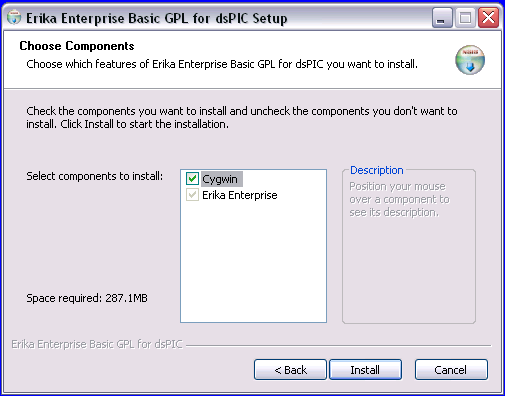
\includegraphics[
  width=8cm, bb=0 0 505 396]{images/installer_options.png}\end{center}
\caption{Questa figura visualizza la dialog box contenente i pacchetti
di installazione disponibili.}
\label{fig:installer-options}
\end{figure}

  \begin{note}
    Il pacchetto di installazione di \ee\ fornisce una versione del
    compilatore C30 di Microchip ricompilato dai sorgenti GCC resi
    disponibili da Microchip. Anche se tale compilatore pu� compilare
    applicazioni C basate su \ee\, esso non include le librerie delle
    periferiche dei dispositivi Microchip, che sono distribuite solo
    con la versione ``ufficiale'' del compilatore C30.
  \end{note}

\item Una volta terminata l'installazione, controllate la {\em prima}
  linea del file che si trova alla locazione
  \file{evidencedir\\bin\\mymake_cygwin.bat} (dove \file{evidencedir}
  � la cartella scelta per l'installazione del sistema). Per esempio,
  se Cygwin � stato installato nella cartella \file{C:\\cygwin},
  allora la prima linea di tale file dovr� essere la seguente:
\begin{lstlisting}
@set EE_BASH_PATH=C:\cygwin\bin\bash
\end{lstlisting}
  ...ovvero, la linea deve contenere il percorso corretto verso il
  file \file{bash.exe} contenuto nella installazione di Cygwin. Se
  avete accettato le cartelle di installazione predefinite
  nell'installer, la cartella corretta deve essere
  \file{C:\\cygwin\\bin\\bash} come specificato nell'esempio
  precedente.
  \begin{note}
    Vi chiediamo di effettuare questa verifica in quanto in alcune
    versioni di Windows l'installer di Cygwin non imposta
    correttamente le chiavi di registro che poi vengono
    successivamente utilizzate dall'installer di \ee\ per la creazione
    del file.
  \end{note}
\end{enumerate}

La restante parte di questo tutorial suppone che Microchip MPLAB IDE
sia installato nella cartella \file{C:\\Programmi\\Microchip} e che lo
GNU Assembler per \dspic\ sia installato nella cartella
\file{C:\\Programmi\\Microchip\\MPLAB ASM30\\ Suite\\bin}. Notate che
questi valori possono essere differenti da quelli presenti sul vostro
PC.

\chapter{Prima esecuzione e configurazione di \rtd}

Dopo aver installato tutti i pacchetti richiesti dal sistema, siete
pronti per eseguire per la prima volta \rtd. Eseguite i seguenti
passi:

\begin{enumerate}
\item Come primo passo, lanciate la Eclipse IDE dal menu Evidence
  all'interno del menu Start, scegliendo
  \file{Start/Programs/Evidence/RT-Druid}.
  
\item Una dialog box apparir� richiedendo la scelta del workspace
  (vedere Figura \ref{fig:select-workspace}).  confermate la directory
  di default, e procedete premendo ``OK''.
%
\begin{figure}[htb]
\begin{center}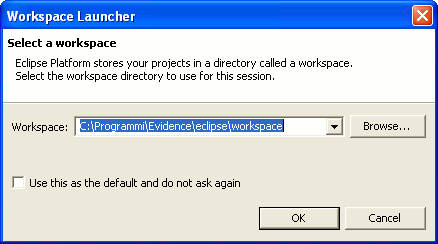
\includegraphics[
  width=12cm, bb=0 0 438 244]{images/select_workspace.png}\end{center}
\caption{Questa figura mostra la dialog box che propone la scelta del
workspace.}
\label{fig:select-workspace}
\end{figure}

\begin{warning}
Il nome della cartella del workspace NON DEVE contenere spazi,
altrimenti \ee\ e \rtd\ potrebbero non funzionare correttamente.
\end{warning}

% ---

\item
  A questo punto, apparir� la finestra di benvenuto di Eclipsee, come
  in Figura \ref{fig:welcome}.
%
\begin{figure}[htb]
\begin{center}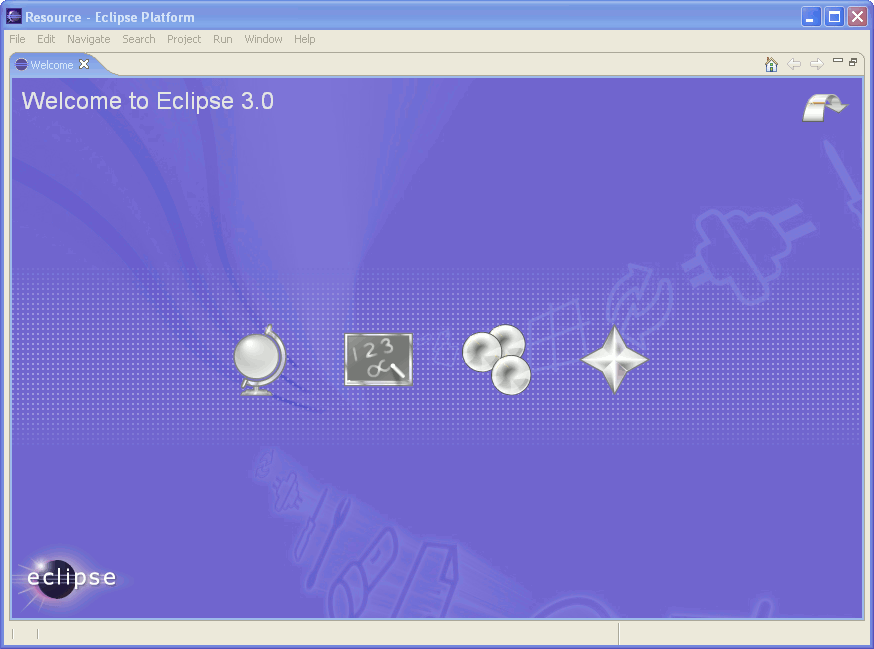
\includegraphics[
  width=12cm, bb=0 0 874 649]{images/welcome.png}\end{center}
\caption{La finestra di benvenuto di Eclipse.}
\label{fig:welcome}
\end{figure}

\item
  Per essere in grado di compilare correttamente un applicativo, �
  necessario indicare correttamente all'interno di \rtd\ la posizione
  del compilatore Microchip C30 e dell'assemblatore Microchip ASM30
  fornito con MPLABIDE.

  Dalla menu ``Preference'', come mostrato in Figura
  \ref{fig:preferences-menu} cercate la scheda ``RT-Druid/Oil/PIC30
  Configurator'' come mostrato in Figura \ref{fig:preferences-pic30}.
  La prima casella di testo, chiamata \const{Gcc path}, fa riferimento
  alla cartella di installazione del compilatore Microchip C30. La
  seconda casella di testo, chiamata \const{Asm path}, fa riferimento
  alla cartella di installazione dell'assemblatore ASM30 fornito con
  MPLAB IDE.

\begin{warning}
Le cartelle di installazione specificate nelle cartelle di testo in
Figura \ref{fig:preferences-pic30} {\em non} includono la cartella
\file{bin}!


Ovvero, \file{c:\\Programmi\\Microchip\\MPLAB C30} � un nome di
cartella corretto, mentre \file{c:\\Programmi\\Microchip\\MPLAB
C30\\bin} non lo �.
\end{warning}

\begin{warning}
La cartella di installazione dell'assemblatore fa riferimento
all'assemblatore ASM30 fornito con MPLAB IDE e {\em non}
all'assemblatore fornito con il compilatore C30. La ragione della
scelta � che la cartella dell'assemblatore � utilizzata sia per
richiamare l'assemblatore sia per copiare il file \file{crt0.s} nella
directory corrente. Deve essere fornita la cartella di ASM30 in quanto
la posizione del file \file{crt0.s} � diversa nelle due versioni di
ASM30 fornite da Microchip (una in MPLAB IDE, una all'interno del
compilatore C30).
\end{warning}

  \begin{figure}[htb]
\begin{center}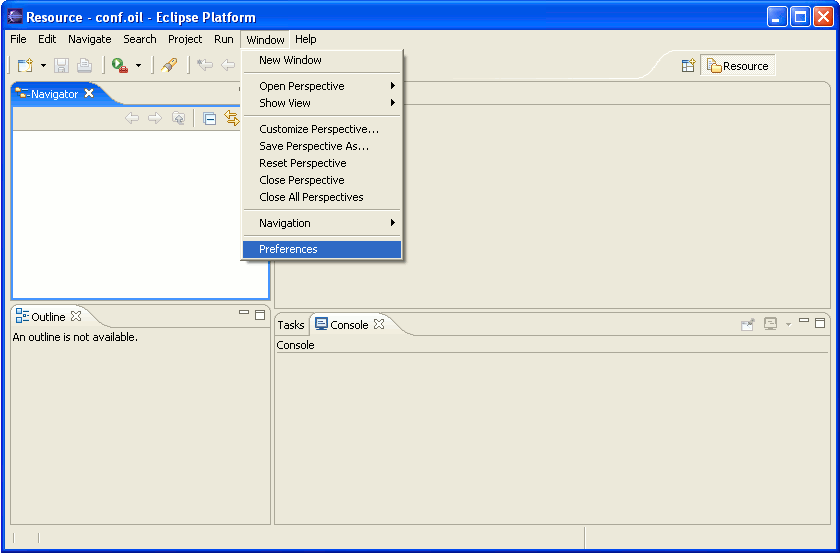
\includegraphics[
  width=12cm, bb=0 0 840 553]{images/preferences_menu.png}\end{center}
\caption{Andate al menu ``Preference''.}
\label{fig:preferences-menu}
\end{figure}

\begin{figure}[htb]
\begin{center}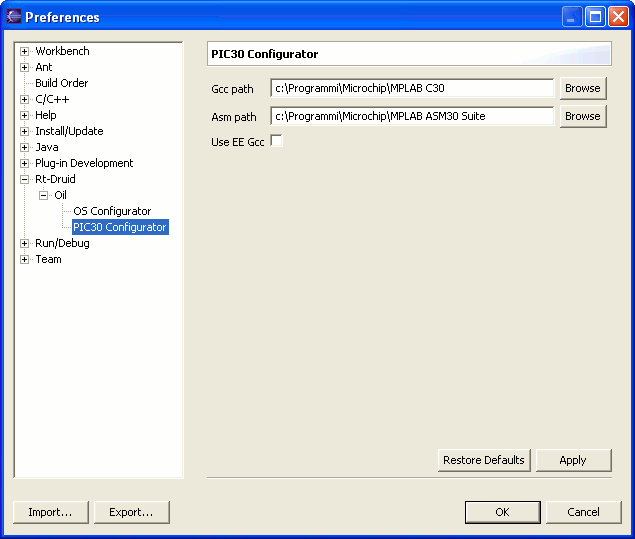
\includegraphics[
  width=12cm, bb=0 0 635 539]{images/preferences_pic30.png}\end{center}
\caption{Specificate le cartelle di instalalzione per il compilatore C30 e per l'assemblatore ASM30 fornito con MPLABIDE.}
\label{fig:preferences-pic30}
\end{figure}

% ---

\item
  Prima di creare e compilare la vostra applicazione, deselezionate la
  voce ``Build Automatically'' nel ``Project'' menu, come visualizzato
  in Figura \ref{fig:build-automatically}.
%
\begin{figure}[htb]
\begin{center}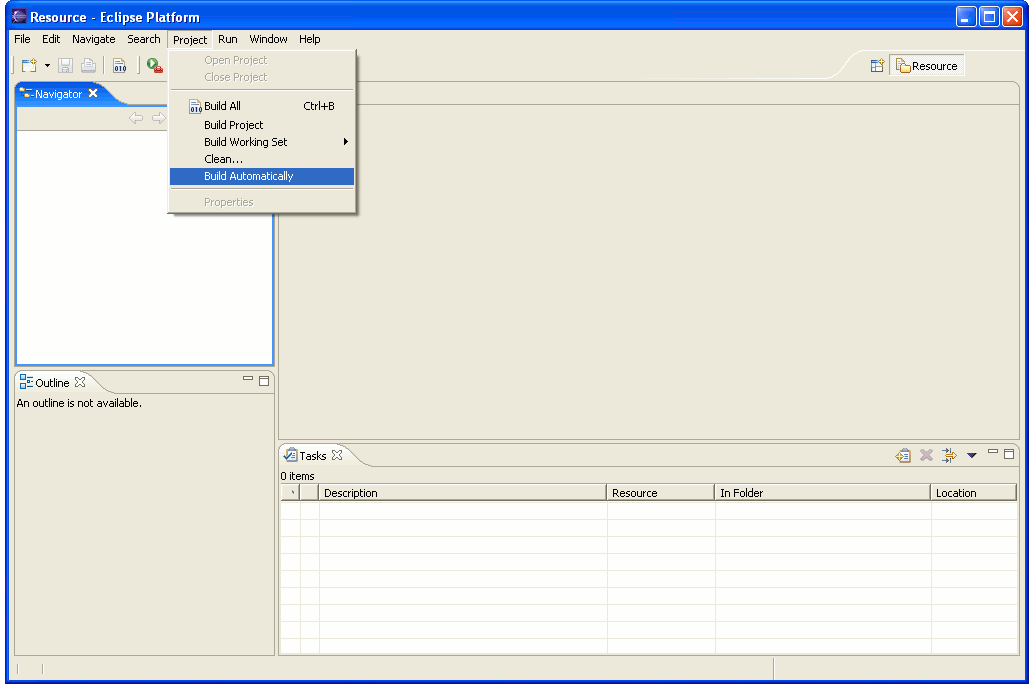
\includegraphics[
  width=12cm, bb=0 0 1029 684]{images/build_automatically.png}\end{center}
\caption{Deselezionate la voce ``Build Automatically'' nel ``Project''
menu.}
\label{fig:build-automatically}
\end{figure}

% ---

% /toOl:
%\item
%  \nb{bla bla bla. bisogna descrivere: la selezione del workpackage, la configurazione delle opzioni di base}

\end{enumerate}

\chapter{Compilare la vostra prima applicazione \ee\ per \dspic}


Siamo a questo punto pronti per compilare la vostra prima applicazione
\ee. Per fare ci�, seguite i seguenti passi:

\begin{enumerate}

\item
  Selezionate ``New Project'', poi ``RT-Druid Oil and c/c++
  Project'' dal ``File menu'', come in Figura
  \ref{fig:new-project}.
%
\begin{figure}[htb]
\begin{center}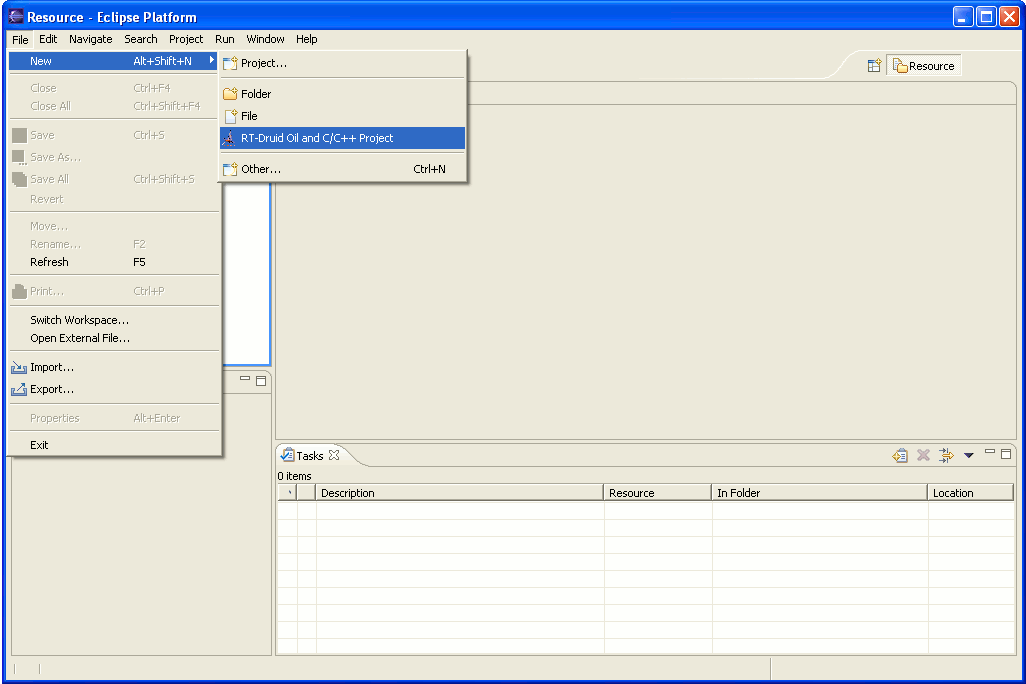
\includegraphics[
  width=12cm, bb=0 0 1026 684]{images/newproject.png}\end{center}
\caption{Selezionate ``New project'' dal ``File'' menu.}
\label{fig:new-project}
\end{figure}

\item
  Apparir� una Dialog box. Selezionate un template per il nuovo
  progetto, come in Figura \ref{fig:new-project2}.
%
\begin{figure}[htb]
\begin{center}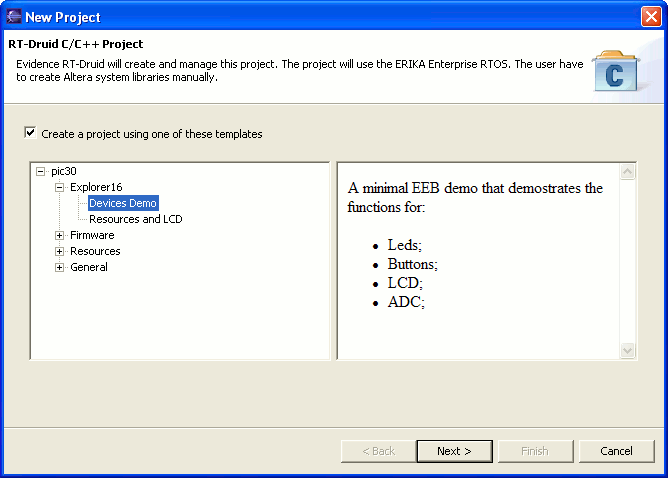
\includegraphics[
  width=12cm, bb=0 0 668 478]{images/newproject2.png}\end{center}
\caption{Selezionate ``RT-Druid Oil and c/c++ Project''.}
\label{fig:new-project2}
\end{figure}

\item
  Premete il bottone ``Next''.

\item
  Inserite il nome del nuovo progetto, ad esempio \const{myProject}
  (ovviamente potete utilizzare nomi diversi), come specificato in
  Figura \ref{fig:projectname}. Premete il bottone ``Finish''.
%
\begin{figure}[htb]
\begin{center}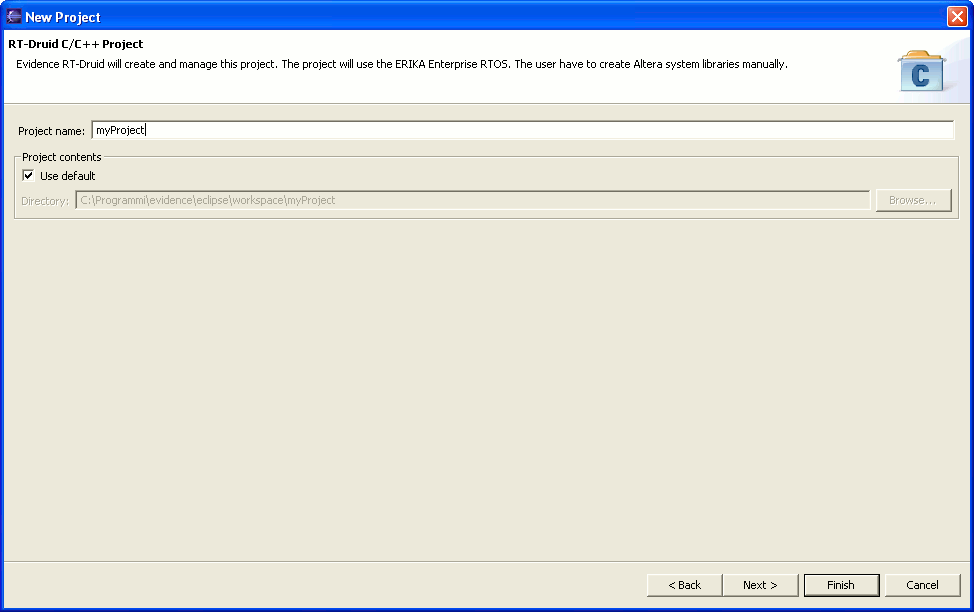
\includegraphics[
  width=12cm, bb=0 0 974 612]{images/projectname.png}\end{center}
\caption{Specificate un nome per il nuovo progetto.}
\label{fig:projectname}
\end{figure}

\item
  Siete a questo punto pronti per compilare l'applicazione. Premete il
  tasto destro del mouse sul nome del progetto nella navigation bar di
  Eclipse, e selezionate ``Build Project''\footnote{``Build Project''
  appare solo se l'opzione ``Build Automatically'' non � selezionata
  nel menu ``Project''.} (vedere Figura \ref{fig:build-project}).
%
\begin{figure}[htb]
\begin{center}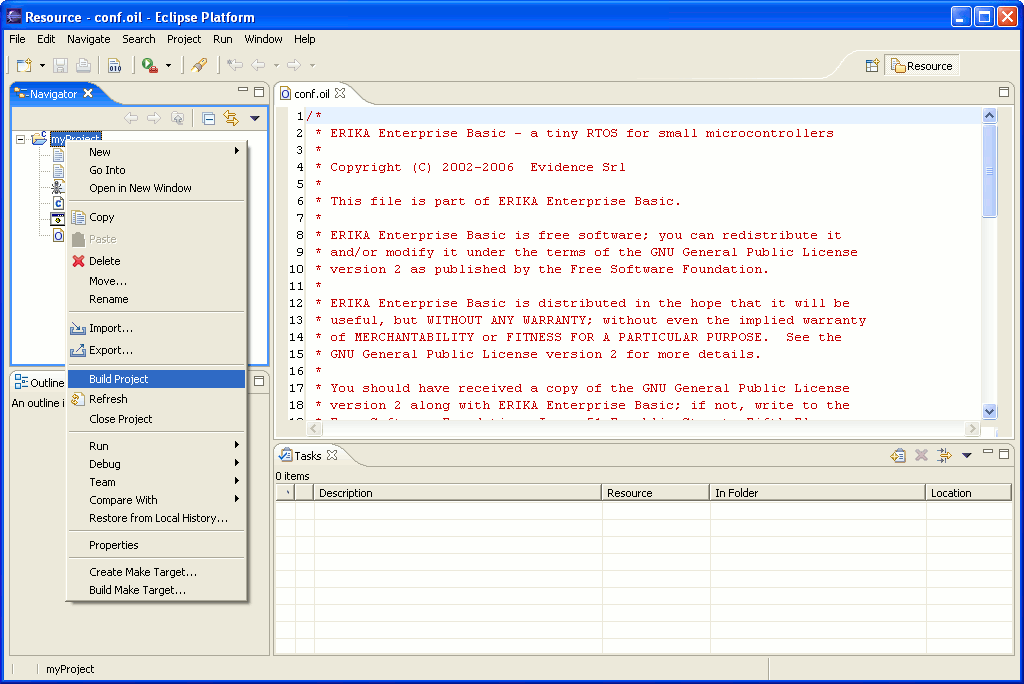
\includegraphics[
  width=12cm, bb=0 0 1024 684]{images/build_project.png}\end{center}
\caption{Adesso � possibile compilare il progetto.}
\label{fig:build-project}
\end{figure}

\item
  A questo punto, il processo di compilazione parte come visualizzato
  in Figura \ref{fig:compiling}.
%
\begin{figure}[htb]
\begin{center}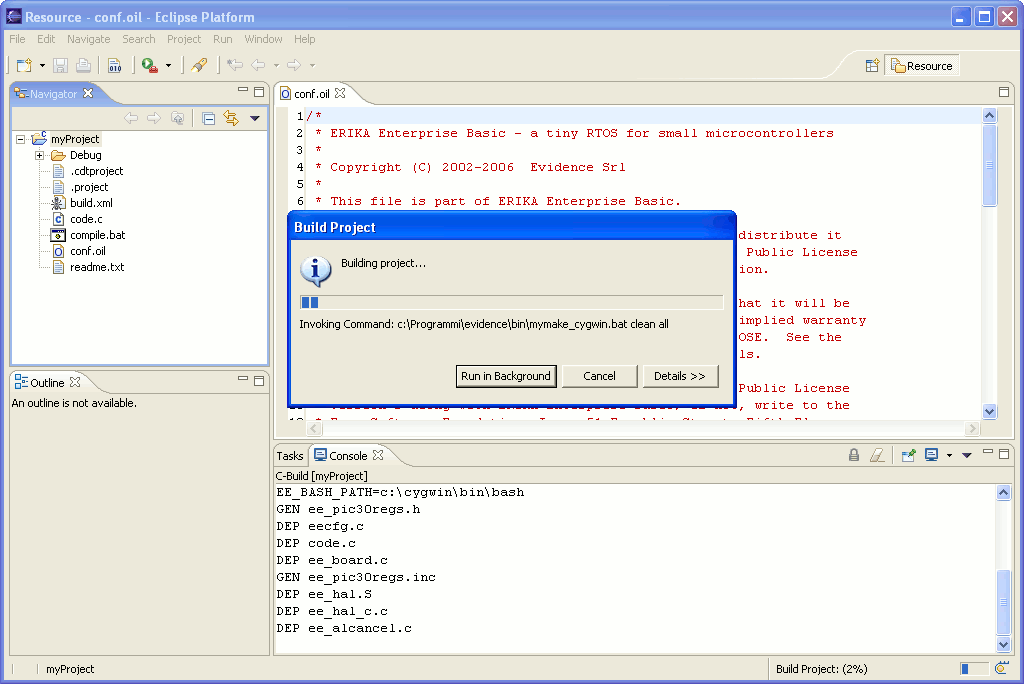
\includegraphics[
  width=12cm, bb=0 0 1024 684]{images/compiling.png}\end{center}
\caption{Il processo di compilazione.}
\label{fig:compiling}
\end{figure}

\begin{note}
  Se appare l'errore visualizzato in Figura
  \ref{fig:mymake_cygwin_error} (ovvero, \file{mymake_cygwin.bat} non
  pu� trovare un file), allora seguite attentamente le istruzioni
  all'ultimo punto del Capitolo \ref{cha:installing}.
\end{note}
%
\begin{figure}[htb]
\begin{center}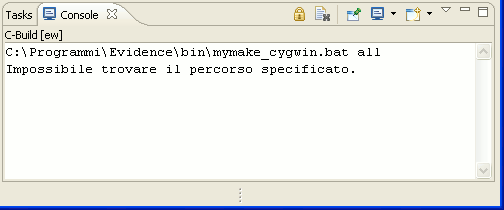
\includegraphics[
  width=12cm, bb=0 0 504 210]{images/mymake_cygwin_error.png}\end{center}
\caption{Un errore che si verifica su alcune macchine Windows. Per
risolvere il problema, controllate il file \file{mymake_cygwin.bat}
come indicato nell'ultimo punto del Capitolo \ref{cha:installing}.}
\label{fig:mymake_cygwin_error}
\end{figure}

\item Alla fine del processo di compilazione viene prodotto un file in
  formato ELF chiamato \file{pic30.elf} all'interno della directory
  \file{Debug} all'interno del progetto, come mostrato in Figura
  \ref{fig:elf-file}. Tale file � il programma eseguibile che pu�
  essere programmato sul device utilizzando MPLABIDE.
%
\begin{figure}[htb]
\begin{center}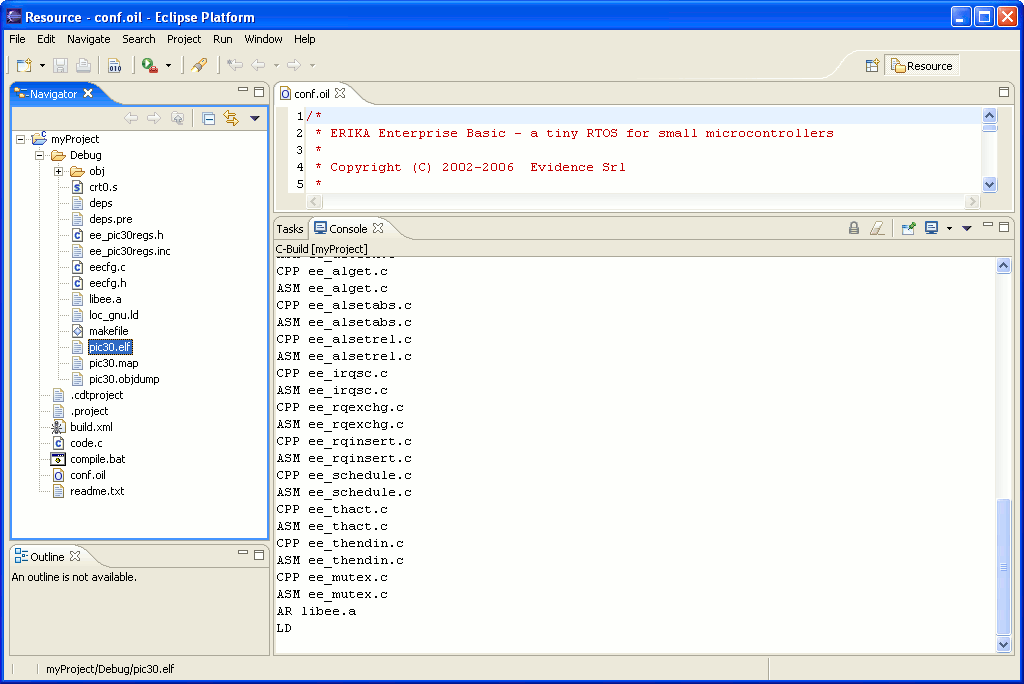
\includegraphics[
  width=10cm, bb=0 0 1024 684]{images/elf_file.png}\end{center}
\caption{\file{pic30.elf} � il file di output che � pronto per essere
programmato sulla scheda target.}
\label{fig:elf-file}
\end{figure}

  
\item
  Il prossimo passo da eseguire riguarda la programmazione del file
  ELF generato durante la compilazione all'interno della scheda
  target. Per fare questo, occorre importare il file ELF all'interno
  del'ambiente di sviluppo Microchip MPLAB IDE. Per fare questo,
  eseguite MPLAB IDE. Apparir� una finestra come quella mostrata in
  Figura \ref{fig:mplab1}.
%
\begin{figure}[htb]
\begin{center}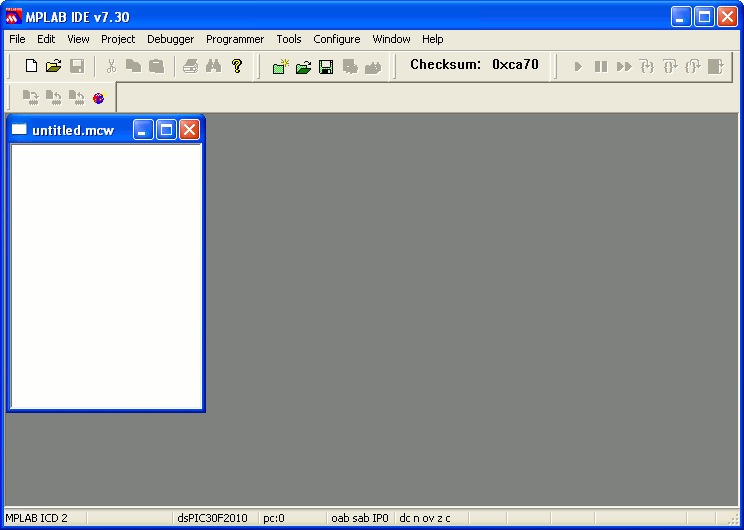
\includegraphics[
  width=12cm, bb=0 0 744 530]{images/mplab1.png}\end{center}
\caption{L'ambiente di sviluppo Microchip MPLAB IDE.}
\label{fig:mplab1}
\end{figure}

\item
  Scegliete ``Import...'' dal menu ``File'', come mostrato in Figura
  \ref{fig:mplab2}.
%
\begin{figure}[htb]
\begin{center}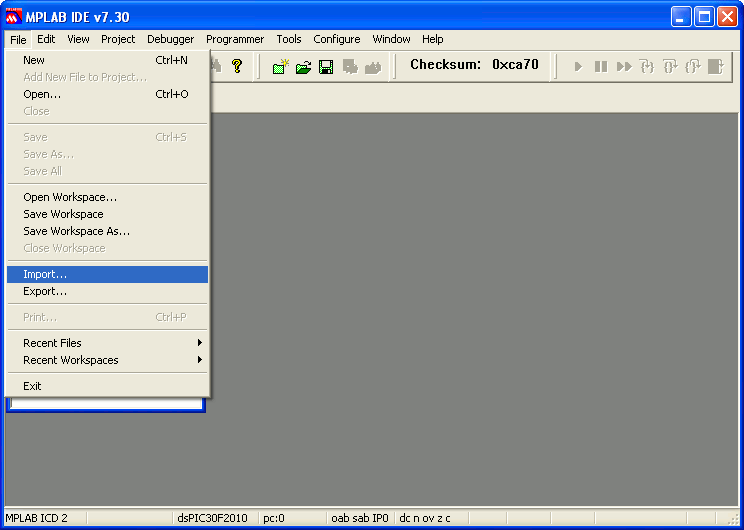
\includegraphics[
  width=12cm, bb=0 0 744 530]{images/mplab2.png}\end{center}
\caption{Scegliete ``Import...'' dal menu ``File'' per importare il
file ELF prodotto da Eclipse.}
\label{fig:mplab2}
\end{figure}

\item
  Apparir� una dialog box. Selezionate il file \file{pic30.elf}
  prodotto dal processo di compilazione in Eclipse, come mostrato in
  Figura \ref{fig:mplab3}. Il file da importare si trova nella
  cartella del workspace che avete specificato all'inizio di questo
  documento in Figura \ref{fig:select-workspace}. In questo esempio,
  il file � memorizzato nella directory
  \file{c:\\Programmi\\Evidence\\eclipse\\workspace\\}
  \file{pic30_oo_mono\\Debug}.
%
\begin{figure}[htb]
\begin{center}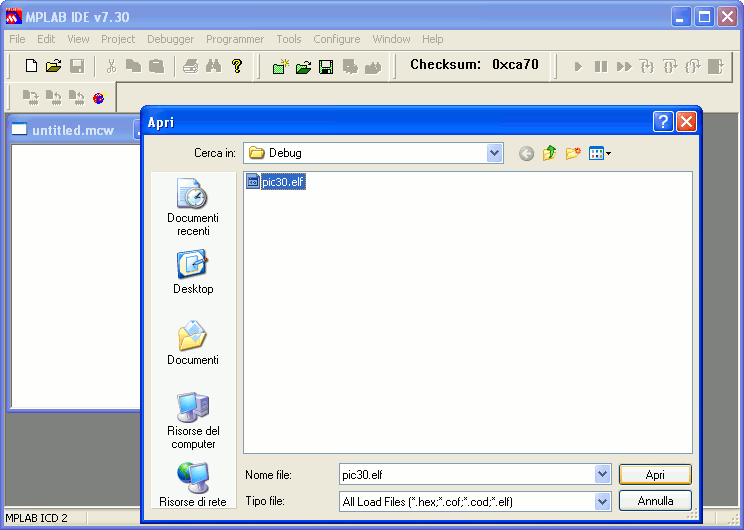
\includegraphics[%
  width=12cm, bb=0 0 744 530]{images/mplab3.png}\end{center}
\caption{Selezionate il file ELF prodotto nel processo di compilazione.}
\label{fig:mplab3}
\end{figure}

\item
  Una volta importato il file ELF all'interno di MPLAB IDE, siete
  pronti per effettuare una sessione di programmazione e debugging
  come normalmente avviene con il software fornito da
  Microchip. Occorre inoltre notare come non ci sia bisogno di creare
  un ``progetto'' di MPLAB IDE, in quanto l'intero processo di
  compilazione � gestito da Eclipse. Ad esempio, Figura
  \ref{fig:mplab4} mostra la finestra ``Disassembly Listing'' e la
  finestra ``Program Memory''. Notate come MPLAB IDE riconosca
  correttamente i simboli di debug del codice sorgente prodotto e
  compilato all'interno dell'ambiente Eclipse.
%
\begin{figure}[htb]
\begin{center}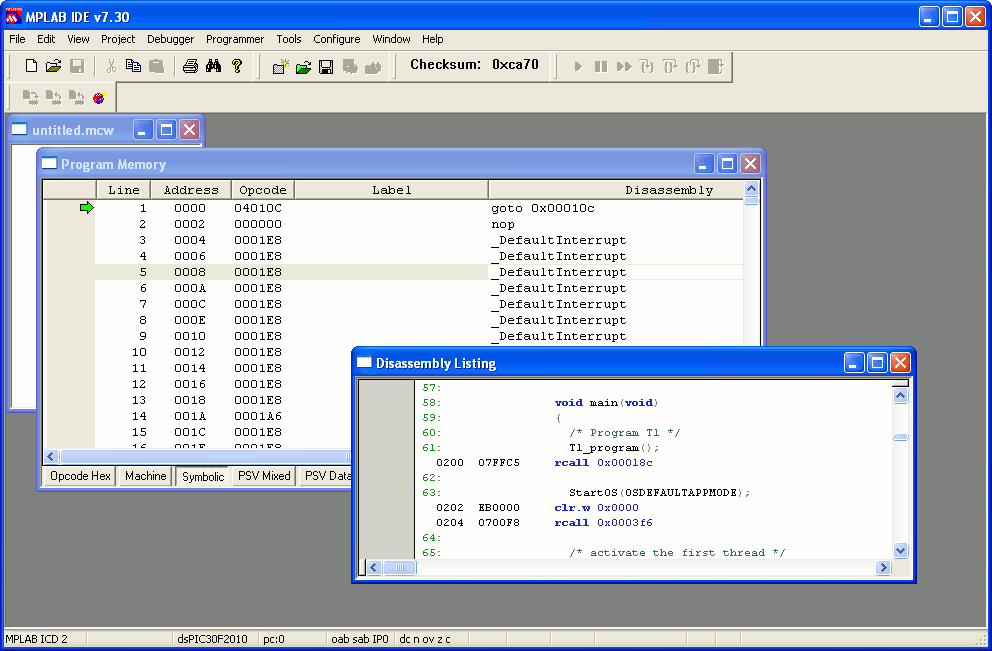
\includegraphics[
  width=12cm, bb=0 0 992 651]{images/mplab4.png}\end{center}
\caption{I simboli di debug sono correttamente riconosciuti da MPLAB IDE.}
\label{fig:mplab4}
\end{figure}

\item
  A questo punto � possibile far partire una sessione di debugging e programmazione per la vostra applicazione demo usando MPLAB IDE.
\end{enumerate}

La Figura \ref{fig:explorer16running} mostra la scheda Microchip
Explorer 16 con in esecuzione il demo presente nel template \file{pic30\\explorer16\\Devices
Demo}. Il demo sfrutta i device a bordo della scheda Explorer 16 per visualizzare sul display LCD la temperatura ambiente letta dal sensore di temperatura.

\begin{figure}[htb]
\begin{center}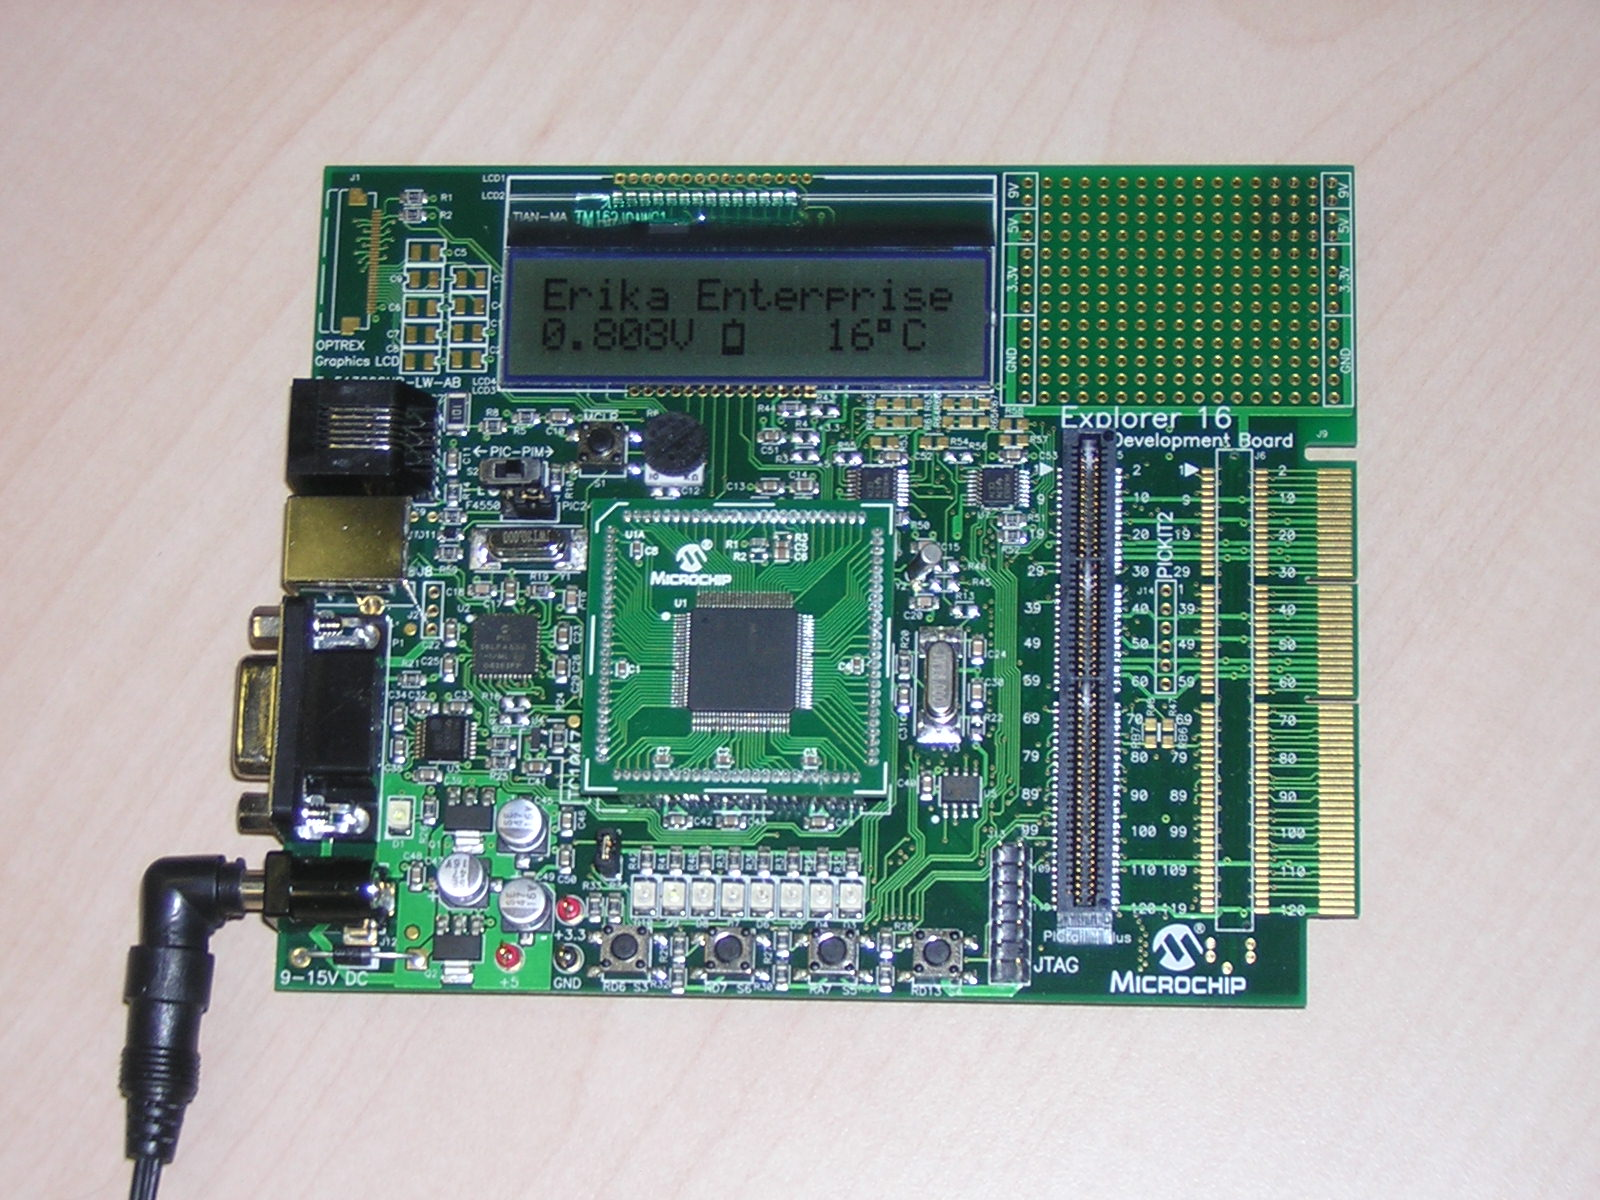
\includegraphics[
  width=12cm, bb=0 0 1600 1200]{images/explorer16running.jpg}\end{center}
\caption{La scgheda Explorer 16 in esecuzione con il programma demo.}
\label{fig:explorer16running}
\end{figure}
